\section{Réalisations}

Cette partie se constitue d'un ensemble de sous-parties décrivant chacune une 
modification que j'ai réalisées sur TCtest. L'ordre chronologique n'est pas 
respecté, en faveur d'un enchainement logique que j'espère plus facile à 
suivre. Par conséquent, ce qui est considéré ici comme une réalisation a pu 
s'écrire de manière itérative tout au long du stage.

Je précise que pendant la première moitié de mon stage, un autre 
stagiaire, Antonin Morelle, a travaillé avec moi sur le programme.

\subsection{Préambule : Technologies et concepts}

TCtest est écrit en Java et construit avec Maven. Eclipse a été utilisé comme 
éditeur. Le code source était géré avec IBM ClearCase et les tâches et bugs 
gérés avec JIRA. Les concepts abordés dans le logiciel sont les suivants :
\begin{itemize}
	\item{orienté-objet}
	\item{multi-threading}
	\item{programmation par interface}
	\item{chargement dynamique et exécution de code externe}
	\item{génération de classe à partir de schémas XML}
	\item{désérialisation d'objet depuis une source XML}
	\item{web services avec Jersey}
\end{itemize}

\subsubsection{JAXB}

JAXB est une API permettant de:
\begin{enumerate}
	\item{générer des classes à partir de schéma XML}
	\item{transformer des fichiers XML en instances de ces classes}
\end{enumerate}
JAXB est très utilisé dans TCtest. C'est un API très pratique puisqu'elle 
permet d'exploiter des données XML de manière très simple. Cependant elle 
est limité par le fait que les classes générées ne peuvent avoir aucun 
comportement. Elles ne contiennent que des accesseurs sur des attributs 
correspondant aux balises \verb|element| du schéma XML.

\subsection{Standardisation des fichiers de configuration}
\label{StandardConfig}

TCtest fonctionne avec deux fichiers de configuration. Un premier 
décrivant l'environnement (dossiers où lire/écrire des ressources), et un 
second décrivant la suite de tests à exécuter, et sur quels ThalesControl les 
exécuter.Dans la version 1.0, le premier était écrit dans ce format :

\begin{verbatim}
TC=C:\TC
Home=C:\TCtest\home
Services=C:\TCtest\services
Tests=C:\TCtest\tests
\end{verbatim}

C'est un format de paires clé-valeur que Java sait lire nativement via la classe
\verb|Properties|. Le second fichier ressemblait à quelque chose de cette 
sorte :

\begin{verbatim}
#WORKFLOW#
workflow1,workflow2,workflow3
#HOME#
tc1,tc2,tc3
\end{verbatim}

C'est un format insolite s'appuyant sur un parser maison. La signification de ce
fichier est la suivante : 
\begin{enumerate}
	\item{Installer les ThalesControl associés aux workflows nommés 
	workflow1, workflow2, et workflow3 dans les dossiers tc1, tc2 et tc3 
	respectivement. Les noms des workflows correspondent à des sous-dossiers du 
	dossier Tests du premier fichier. Les noms des instances de ThalesControl 
	correspondent à des sous-dossers du dossier Home du premier fichier.}
	\item{Exécuter les tests décrit dans les workflows workflow1, workflow2, et 
	workflow3.}
\end{enumerate}

Il m'a semblé superflu d'avoir 2 formats différents, surtout que du XML était 
déjà utilisé pour écrire les workflows (voir partie \ref{CompactWorkflow}). J'ai donc 
réécrit ces fichiers en XML et j'ai utilisé JAXB pour les lire et les 
transformer en objet Java exploitables.

\subsection{Restructuration des fichiers de configuration}

On peut remarquer dans la partie \ref{StandardConfig} qu'un workflow est associé à une 
instance de ThalesControl. Ceci n'a pas de sens. On peut très bien vouloir 
exécuter une même séquence d'action (un même test) sur des instances 
différentes. J'ai donc découpler les workflows des définitions d'instances de 
ThalesControl. Cela s'est traduit par beaucoup de modifications dans le code 
cherchant, lisant, et traitant les fichiers de configuration.

\subsection{Externalisation des connaissances des extensions Hudson}

Un des services déjà disponibles quand je suis arrivé permettait de valider une
extension Hudson en téléchargeant la configuration XML d'une tâche Hudson donnée
utilisant cette extension, puis en extrayant la portion de configuration se 
rapportant à l'extension, et enfin en validant cette portion avec un schéma 
fourni par l'utilisateur. Ce service est utile lorque l'on veut vérifier 
qu'une nouvelle version d'une extension s'insère bien dans les tâches de notre 
Hudson (ou la même extension dans une version différente de Hudson).

Le problème avec ce service est que pour détecter la portion de configuration
XML intéressante, il faut connaitre à l'avance la balise XML racine qui contient
tout ce que l'extension ajoute. Au départ, cette connaissance se trouvait dans 
le code Java, sous forme d'un dictionnaire. Afin de pouvoir supporter de 
nouvelles extensions sans avoir à recompiler, j'ai extrait la connaissance dans 
un fichier XML.

\subsection{Rédaction de workflow plus compact}
\label{CompactWorkflow}

Voici un exemple de workflow pour TCtest 1.0 :

\begin{verbatim}
<Workflow>
  <Id>myid</Id>
  <Target>Hudson</Target>
  <Services>
    <Service>
      <Jar>CreateJob.jar</Jar>
      <Parameters>
        <Parameter>
          <Name>JobName</Name>
          <Value>TheJob</Value>
        </Parameter>
        <Parameter>
          <Name>ConfigFile</Name>
          <Value>configs\config-myid.xml</Value>
        </Parameter>
      </Parameters>
    </Service>
    <Service>
      <Jar>DeleteJob.jar</jar>
      <Parameters>
        <Parameter>
          <Name>JobName</Name>
          <Value>TheJob</Name>
        </Parameter>
      <Parameters>
    </Service>
  </Services>
</Workflow>
\end{verbatim}

C'est beaucoup pour un si petit workflow (seulement 2 services avec chacun 1 ou 
2 paramètres). XML est dense en général, mais ici beaucoup de choses sont 
inutiles. En essayant de réduire la masse de code à écrire, je suis parvenu à 
ce résultat bien plus lisible :

\begin{verbatim}
<workflow>
  <service>
    <jar>CreateJob.jar</jar>
    <parameter name="JobName" value="TheJob"/>
    <parameter name="ConfigFile" value="TheJob"/>
  </service>
  <service>
    <jar>DeleteJob.jar</jar>
    <parameter name="JobName" value="TheJob"/>
  </service>
</workflow>
\end{verbatim}

En plus de faciliter la rédaction de workflow, cette version plus compacte à 
l'avantage de simplifier le code Java qui exploite ces données (je rappelle 
qu'une classe Workflow est générée à partir de la XSD correspondant à ce fichier 
XML).

\subsection{Rapports de résultats}
\label{Reporting}

TCtest 1.0 laissait au service le soin d'écrire leurs propres résultats dans 
des fichiers, où ceux-ci le souhaitaient. J'ai considéré que c'était insuffisant
car du point de vu de l'utilisateur, un test est formé de la séquence de 
services, pas d'un service en particulier. Lors d'une batterie de tests, il 
faut pouvoir répérer tout de suite s'il y a eu une erreur ou si tout est au 
vert.

J'ai donc écrit une API permettant d'ajouter à TCtest des générateurs de rapports.
Ces générateurs sont appelés lorsque tous les tests ont tourné et que les 
résultats ont été collectés. Le modèle de cette API suit celui de l'API des 
services et jouit de la même modularité.

En plus de l'API j'ai dévelopé des générateurs pour les formats suivants:
\begin{description}
	\item[TUSAR]{(Thales Unified Software Analysis Report) est un format XML qui peut 
	(entre autres) exprimer des résultats de tests en 3 états (le test passe, 
	le test échoue, ou erreur lors de l'exécution).}
	\item[RST]{est un langage utilisé pour écrire des documents, et qui peut 
	être compilé en HTML, LaTeX, OpenOffice ou encore Word. Il est utilisé dans 
	l'équipe ThalesControl pour écrire la documentation des produits. Je l'ai 
	choisi car j'ai ainsi pu écrire un seul générateur pour de multiples formats
	de sortie finaux.}
\end{description}

\subsection{Service de validation du statut d'une tâche Hudson}
\label{BuildSuccessService}

Il était indispensable d'avoir un service permettant de savoir si une tâche 
Hudson donnée a été exécutée avec succès ou non. Comme tous les autres services
interragissant avec Hudson, la communication avec le scheduler se fait via son
interface web service, autrement dit par des requête HTTP. La librarie Jersey 
a été utilisé pour cela.

\subsection{Service de validation de la sortie standard d'une tâche Hudson}

Lorsqu'Hudson exécute une tâche, un journal est écrit. Ce journal joue le 
rôle de sortie standard pour les programmes que la tâche lance (Maven par 
exemple). Il est récupérable via une requête HTTP sur le serveur hébergeant 
Hudson. J'ai donc écrit un service qui assure qu'une première expression 
régulière donnée se trouve bien dans le journal, et qu'une deuxième ne s'y 
trouve pas. Un cas typique d'utilisation de ce service est de lui fournir 
en paramètre \verb|(SUCCESS, FAILURE)|, car les journaux des tâches Hudson 
sont toujours clos par l'un ou l'autre de ces mots. Dans ce cas de figure le 
service remplit exactement la même fonction que le service décrit en 
\ref{BuildSuccessService}. Des expressions régulières bien plus complexe sont 
bien sûr acceptées, d'où l'utilité du service.

\subsection{Service d'extraction du schéma et des données d'une base de données}
\label{DbExtraction}

Afin d'étudier la base de données de Sonar (voir partie \ref{ProbSonar}), il 
m'a été demandé d'écrire deux services visitant une base de données pour en 
extraire le shéma ou les données. Je me suis appuyé pour cela le projet Apache 
DB DdlUtils. La sortie de ces services est un fichier Turbine XML contenant le 
schéma ou les données. Turbine XML est un langage capable de décrire un 
schéma ou des données indépendamment de l'implémentation de la base de données
sous-jacente (MySQL, Oracle, Microsoft SQL...). Il est utilisé dans d'autres 
projets de la fondation Apache tel que l'object relational mapper Torque, 
lui-même composant du framework de développement web Turbine.

\subsection{Service de comparaison de fichiers}

Toujours dans la perspective d'étudier Sonar, le besoin s'est exprimé de pouvoir 
comparer la base données entre deux versions de Sonar. Sachant que je disposait
des deux services décrit en partie \ref{DbExtraction}, je n'avais plus qu'à 
comparer des fichiers XML. J'ai donc développé un 
service permettant de comparer deux fichiers selon la méthode ligne par ligne 
dite \textit{unified diff}, c'est-à-dire la méthode standard dans nombre de 
logiciel, y compris la fameuse commande \verb|diff|. La bibliothèque 
Java-Diff-Utils a été utile pour cela.

\subsection{Amélioration de l'intégration de l'installateur ThalesControl}

ThalesControl étant hautement personnalisable, on ne peut pas savoir à l'avance 
comment démarrer une instance. Pour certaines instances le démarrage consiste 
à démarrer des serveurs Tomcat, pour d'autres une base de données Derby ou 
Oracle. Pourtant TCtest 1.0 se basait uniquement sur les instances ThalesControl
"demo" (Tomcat + Derby) et était incapable de démarrer d'autres type 
d'instances.

Par conséquent, j'ai étudié l'installateur de plus près et ai pu constater 
qu'à la fin de l'installation, un fichier de log est écrit, dans lequel on peut 
trouver une liste des URL des serveurs de l'instance installée ainsi qu'une 
liste des commandes exécutables sur l'instance pour la démarrer et l'arrêter.
Fort de cette trouvaille j'ai programmé dans TCtest un analyseur pour ce fichier
journal. L'analyseur en question est entièrement écrit dans une classe séparée 
et se base sur 6 expressions régulières pour détecter les données intéressantes.
Par conséquent, si une version future de l'installateur vient à produire le log
de manière différente, il sera très simple d'adapter l'analyseur, soit en 
modifiant les expressions régulières, soit en réimplémentant la classe. 

Ma version de TCtest est donc capable de s'adapter à un ensemble 
d'instance beaucoup plus grand, si ce n'est toutes les instances.

\subsection{Exploitation d'instances de ThalesControl déjà lancées}

Thales a besoin que TCtest puisse faire tourner ses tests sur des instances 
de ThalesControl déjà installées et opérationnelles. TCtest 1.0 n'a pas cette 
fonctionnalité. Si ce n'est pas TCtest qui installe ThalesControl, alors on 
ne peut pas savoir la structure de l'installation (comment sont rangés les 
fichiers ?) ni l'adresse du ou des serveurs, car on n'a pas les fichiers de 
configuration qui ont généré l'installation, voire l'installation a pu se faire 
manuellement (sans l'installateur).

Par conséquent, si l'utilisateur souhaite utiliser des instances pré-installées, 
il doit fournir les adresses des serveurs manuellement. Le besoin de pouvoir
spécifié toutes les infos sur une instance de ThalesControl (autre que celles 
propres à l'installateur) s'est alors fait sentir. A nouveau j'ai fait appel à 
XML.

\subsection{Préchargement des extensions}

Dans la version 1 de TCtest, les services doivent être instancié à chaque fois 
qu'ils sont utilisés. Par exemple si un service est appelé 4 fois dans un 
workflow et que ce workflow est lui-même appelé 5 fois lors d'une batterie de 
tests alors le service sera instancié 20 fois. Cela peut être coûteux si il 
faut lire un fichier ou se connecter à une base données. De plus, dans 
l'implémentation 1.0, c'est toute la libraire du service qui est rechargé.

Pour résoudre ce problème il m'a fallu séparer les paramètres des services
en deux catégories : les paramètres d'initialisation (constructeur) et les 
paramètres d'exécution (méthode \verb|execute|). Par exemple pour les services 
d'extraction de base de données (voir partie \ref{DbExtraction}), un paramètre 
d'initialisation est l'emplacement des pilotes JDBC tandis qu'un paramètre 
d'exécution est l'URL de la base à extraire. Mais comment fournir les paramètres
d'initialisation ? La solution choisie a été de les placer dans un fichier 
XML portant le même nom que le fichier JAR du service correspondant, et placé
dans le même dossier.

Ainsi TCtest parcoure le ou les dossiers contenant des extensions (indiqué 
dans le fichier de configuration de l'environnement), charge les JAR qu'il 
trouve dedans et instancie les classes compatibles. Les instances résultantes 
sont ensuite stockées dans un structure de type dictionnaire (la clé étant 
le nom du fichier JAR sans l'extension), prêtes à être utilisées en cas de 
référence dans un workflow.

\subsection{Réécriture de l'API}
\label{NewAPI}

Un service pour TCtest 1.0 est constitué d'une collection de classe dont une 
respecte l'interface \verb|Service|, qui ne contient qu'une méthode, 
\verb|execute|. Cette méthode n'a ni paramètres ni valeur de retour, et peux
lever toute exception de type \verb|Exception|.
Les paramètres du service sont passés au constructeur de la classe.

Cette interface est nettement insuffisante. J'ai repertorié les problèmes 
qu'elle pose :
\begin{itemize}
	\item{Les paramètres sont passés au constructeur mais ne soit exploités 
	que dans \verb|execute|, ce qui amène à copier toutes les valeurs dans des 
	attributs de la classe du service et donc à du code supplémentaire inutile.}
	\item{Le nombre de paramètres et leurs types sont fixes. Il n'y aucune 
	flexibilité sur la quantité de données que l'on peut fournir à un service. 
	Ceci empêchait les fonctionnalités décrites en \ref{TestTree}.}
	\item{Sans valeur de retour, la seule chose que l'on peut savoir sur 
	l'exécution d'un service est si une exception a été levée ou non. Ce n'est 
	pas suffisant puisque ce que l'on veux, c'est tester. On veut pouvoir 
	obtenir un résultat disant si le test passe ou pas (dans ces deux cas, 
	aucune exception n'est levé puisque c'est le fonctionnement normal du 
	service que de renvoyer ce résultat).}
	\item{La signature de \verb|execute| lui permet de lever quasiment 
	n'importe quelle exception. Ceci permet au développeur du service de se 
	passer complètement de structures try-catch. Cela peut être vu comme un 
	avantage, mais cela vient également avec un inconvénient : les exceptions 
	remontent à l'appelant sans aucun contexte, voir sans même que le 
	développeur se rende compte qu'une erreur peut se produire dans son code !}
\end{itemize}

J'ai résolu les 4 derniers problèmes en créant une nouvelle interface offrant un 
maximum de flexibilité pour de futures amélioration :

\begin{verbatim}
public interface ExtensionTask {
  Result run(Context context);
}
\end{verbatim}

\verb|Result| et \verb|Context| sont des interfaces. 

\verb|Context| encapsule 
des paires nom-valeur accessible via la méthode 
\verb|<T> T getVar(String name)| On peut donc passer un nombre potentiellement
illimité de paramètre à \verb|run|. Cette interface n'a pas d'implémentation 
dans l'API, seulement dans le lanceur.

\verb|Result| encapsule le résultat d'une 
méthode de test. Ceci est visible par les méthodes \verb|isSuccess()|, 
\verb|isFailure()| et \verb|isError()|. En plus de cela cette interface expose
les méthodes \verb|getMessage()| qui retourne un message (\verb|String|) 
expliquant ou détaillant le résultat, et \verb|getError()| qui retourne 
l'exception levée par la méthode s'il y a lieu (\verb|null| si pas d'exception).
L'unique implémentation disponible de cette interface dans l'API 
(\verb|ExtensionResult|) n'expose pas 
de constructeur, mais des méthodes statiques retournant un objet de type 
\verb|Result|. Ces méthodes sont \verb|success()|, \verb|failure()| et 
\verb|error(Throwable t)|. Chacune des trois méthodes dispose d'une surcharge 
proposant de passer un message en plus. Comme \verb|run| n'a plus de clause 
\verb|throws|, le développeur de service se voit forcer de gérer correctement
les exceptions de son code et de retourner un résultat. S'il tente de retourner
\verb|null|, le lanceur émettra un message d'erreur expliquant que \verb|null| 
n'est pas accepté et quittera. Le lanceur est aussi protégé contre tout service 
codé incorrectement par une structure \verb|throw-catch(Throwable)|, ce qui 
n'était pas le cas du lanceur 1.0.

On remarquera l'abandon du nom "service" au profit de "extension". Ceci est du 
au fait que j'ai fusionné l'API des services avec celles de générateurs de 
rapport (partie \ref{Reporting}). L'interface \verb|ExtensionTask| pourra 
être utilisée dans le cas où de nouveaux types d'extension TCtest sont 
imaginés. Tout le code gérant le chargement des fichiers JAR des extensions et
leur exécution dans la lanceur a été factorisé.

\subsection{L'arbre des tests}
\label{TestTree}

Dans un workflow pour TCtest 1.0, il est impossible de partager un paramètre 
entre plusieurs services. Pourtant cette fonctionnalité est extrêmement utile.
Par exemle quand on a une séquence de services travaillant sur une même tâche 
Hudson, le valeur du paramètre \verb|JobName| est la même pour tous les services
(voir l'exemple de workflow en \ref{CompactWorkflow}). Il était donc intéressant
de pouvoir assigner des 
paramètres à l'échelle du workflow. Et si on voulait utiliser la même séquence 
de services, mais avec un autre nom de tâche ? Alors il faudrait pouvoir 
assigner des paramètres au niveau du test, mais à l'extérieur du workflow. 
On pourrait même vouloir partager des paramètres entre plusieurs workflows.
Et enfin comment effectuer plusieurs tests sur une instance de ThalesControl
sans avoir à le répéter pour chaque test ?

Afin de rendre tout cela possible, il m'a fallu réimplémenter une grande partie 
du lanceur. En effet l'architecture de la version 1.0 (au niveau organisation 
du code) ne permet en aucun cas d'ajouter ce genre
de fonctionnalités. En particulier, alors que Java est un langage très orienté 
objet, TCtest 1.0 n'en prenait pas partie. Un programme objet
comprend des classes pour réprésenter les types d'objets qu'il manipule, mais 
TCtest 1.0 comprend des classes telles que \verb|Tool|, \verb|TestConfig|, 
\verb|InstallManager|, \verb|Launcher| etc. qui n'ont pas vraiment de sens dans 
l'environnement de TCtest. On devrait plutôt trouver des classes telles que 
\verb|ThalesControl|, \verb|Test|, \verb|TestSuite|, \verb|Service| etc.

Je suis donc reparti de zéro afin de trouver une architecture je l'espère plus 
sensée et 
extensible. Les fonctionnalités à implémenter impliquent un ensemble d'objets
où chacun à un parent (un service à pour parent un workflow) et des enfants
(un workflow a plusieurs services enfant). J'ai donc pensé à un arbre, 
représenté en figure \ref{TestTreeFig}. A cet arbre on peut attacher des 
instances de ThalesControl (instances de la classe \verb|ThalesControl|) et des 
paramètres. Les noeuds héritent de leur parent tous les paramètres ainsi que 
l'instance de ThalesControl. Cette architecture est expliquée avec précision 
dans le manuel utilisateur en annexe.

\begin{figure}[htb]
	\centering
	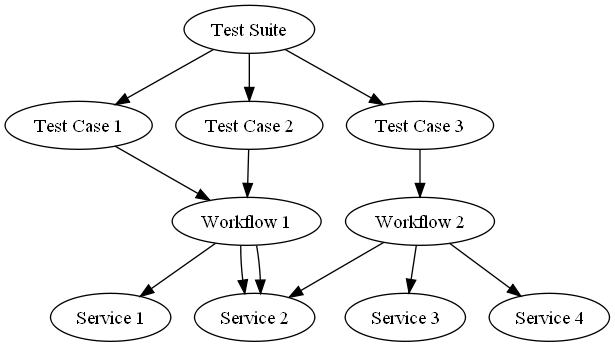
\includegraphics[scale=0.6]{test_tree.png}
	\caption{L'arbre de test}
	\label{TestTreeFig}
\end{figure}

L'arbre des tests est complètement retranscrit dans mon code. Chacun des types
d'objet correspond à une classe. Cependant j'ai conçu ces classes afin que 
l'arbre puisse devenir plus complexe. Ainsi toutes ces classes implémentent
l'interface \verb|Test|, ou l'interface \verb|TestSuite|, qui hérite de 
\verb|Test|. Ces deux interfaces se présentent ainsi (pour la description des 
interfaces \verb|Context| et \verb|Result| qui apparaissent \verb|Test|, voir 
partie \ref{NewAPI}) :

\begin{verbatim}
/**
 * The root interface for all of the test objects.
 * @author Hugo Wood
 */
public interface Test extends Runnable {
  
  /**
   * Returns the context of the test. The context acts as the input value of 
   * the run method and therefore should not be null before the {@link run} 
   * method is called.
   */
  Context getContext();

  /**
   * Returns the result of the test. The result acts as the output value of 
   * the run method and therefore should not be null after the {@link run} 
   * method has been called.
   */
  Result getResult();
   
}

/**
 * A test that contains other tests.
 * @author Hugo Wood
 */
public interface TestSuite extends Test, Iterable<Test> {
  
  /**
   * Returns the number of tests in this suite.
   */
  int getSize();

}
\end{verbatim}

Par conséquent, un service est un test, et un workflow une test suite. 
L'extensibilité vient du fait que via ce système d'interface, différentes 
implémentations peuvent cohabiter. Et c'est déjà le cas dans mon code puisque 
les classes \verb|SequentialTestSuite| (test suite qui exécutent ses tests en 
série) et \verb|ParallelTestSuite| (en parallèle) sont bien deux implémentations
différentes de \verb|TestSuite|. Un diagramme des classes simplifié de TCtest 5 
(la version que j'ai laissé en partant) est présenté en figure \ref{Classes}.
Notons en passant que \verb|Test| hérite de \verb|Runnable|, ce qui rend les 
objets de l'arbre facilement utilisables avec l'API \verb|java.util.concurrent| 
pour le multi-threading.

\begin{figure}[htb]
	\centering
	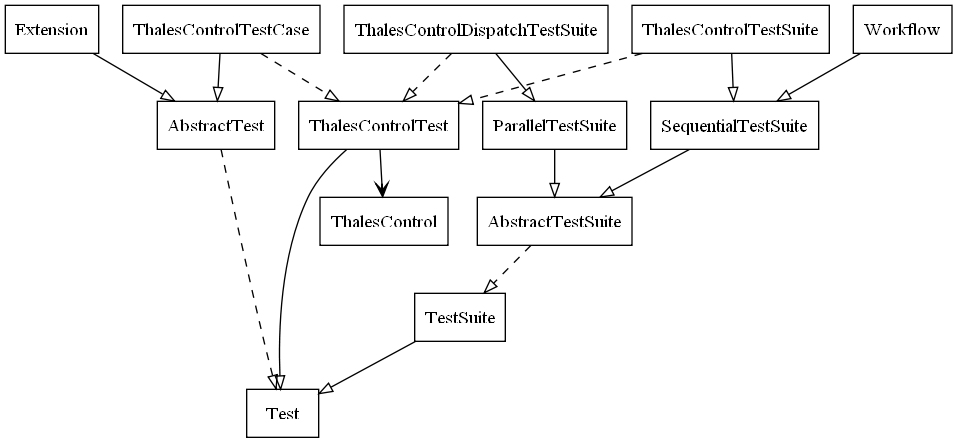
\includegraphics[scale=0.4]{classes.png}
	\caption{Diagramme des classes}
	\label{Classes}
\end{figure}

A \verb|Test| et \verb|TestSuite| vient s'ajouter l'interface 
\verb|ThalesControlTest| qui est simplement un test qui contient un objet de 
type \verb|ThalesControl|. On devine le rôle de chaque classe avec son nom et 
les classes dont elle hérite (mise à part \verb|ThalesControlDispathTestSuite|, 
décrite en \ref{ReParallel}).

\subsection{Reparallélisation}
\label{ReParallel}

Comme décrit en \ref{Parallel}, TCtest 1.0 est une application multi-threadée.
Cependant la parallélisation n'est pas optimale. En effet, elle n'autorise 
qu'un seul test à la fois, alors que la véritable contrainte est que l'on ne 
peut exécuter qu'un seul test à la fois \textit{par instance de ThalesControl}. 
J'ai donc écrit la classe \verb|ThalesControlDispathTestSuite| (voir le 
diagramme des classes en \ref{TestTree}). Les instances de cette classe 
analysent entièrement à l'avance l'ensemble 
des tests qu'elles ont à effectuer, déterminent les instances de ThalesControl qui 
vont être utilisées, créent un thread par instance, et enfin distribuent
les tests sur les différents thread suivant l'instance à laquelle ils sont 
destinés. L'avantage de cette méthode, outre son efficacité, est que son 
implémentation ne requiert pas de communications entre les threads. Le programme 
est donc bien plus robuste.

\subsection{Protection contre une configuration mal-formée}

TCtest 1.0 ne se protégeait quasiment pas contre des fichiers de configuration 
mal-formés. Comme j'avais standardisé tous les fichiers de configuration en 
les écrivant au format XML et utilisant JAXB pour les exploiter, j'ai pu 
centraliser dans une seule classe le code permettant de transformer une fichier 
XML en un objet complet avec comportement. Concrètement cette classe lit 
les fichiers de configuration avec JAXB, en tire des pseudo-objets réprésentant 
le contenu des fichiers, vérifie que ce contenu est valide, puis construit à 
partir du contenu des instances des classes de l'arbre de test, notemment des 
instances de \verb|ThalesContrlol|, \verb|ThalesControlTestCase|, 
\verb|Workflow| et \verb|ThalesControlDispatchTestSuite|.

En cas d'erreur dans l'étape de vérification, un message d'erreur est envoyé à 
l'utilisateur avec suffisamment de détails pour qu'il puisse corriger le fichier
de configuration incriminé.

\subsection{Manuel utilisateur}

J'ai écrit un manuel complet pour l'utilisateur de TCtest. Il en décrit le 
principe, comment en tirer parti ainsi que la manière dont les fonctionnalités
peuvent être étendues. Comme toute documentation produite par Thales CST, le 
manuel est écrit en Anglais. Une copie se trouve en annexe.